\documentclass[10pt,letterpaper]{article}
\usepackage[margin=0.85in]{geometry}
\usepackage{amsmath,amssymb}
\usepackage{microtype}
\usepackage{hyperref}
\usepackage{graphicx}
\usepackage{subcaption}
\usepackage{titlesec}
\titleformat{\section}{\large\bfseries}{\thesection}{0.6em}{}
\titlespacing*{\section}{0pt}{0.7em}{0.3em}
\titleformat{\subsection}{\normalsize\bfseries}{\thesubsection}{0.5em}{}
\titlespacing*{\subsection}{0pt}{0.5em}{0.2em}
\setlength{\parskip}{0.25em}
\setlength{\parindent}{0pt}

\title{\vspace{-1.2cm}\textbf{An FFT-Based Real-Time Ocean Surface Simulator}\\
\large CS 384P Final Project Report}
\author{Will Suan}
\date{April 29, 2026}

\begin{document}
\maketitle
\vspace{-1.0cm}

\section{Algorithms}

\subsection{Overview}
This project simulates a wind-driven ocean surface in real time using the
statistical FFT model of Tessendorf~\cite{tessendorf}. The surface elevation
is treated as a stationary random field whose Fourier components are sampled
from the Philips wave spectrum and evolved in time using the deep-water
dispersion relation. Heights are recovered each frame by a 2D inverse FFT.
On top of that we add: (i) a horizontal displacement field that produces
sharp Gerstner-like crests, (ii) a foam mask derived from the Jacobian of the
displacement field, and (iii) a 3-layer cascade with coprime patch sizes
that hides the periodicity of any single FFT.

\subsection{Philips spectrum and Fourier representation}
We represent the surface elevation $h(\mathbf{x},t)$ on a square patch of
side $L$ as a sum of Fourier modes with wave-vectors
$\mathbf{k}=(k_x,k_z)=2\pi(n,m)/L$ for $n,m\in[-N/2,N/2)$:
\begin{equation}
  h(\mathbf{x},t) \;=\; \sum_{\mathbf{k}} \tilde{h}(\mathbf{k},t)\,e^{i\mathbf{k}\cdot\mathbf{x}}.
  \label{eq:fourier}
\end{equation}
Initial spectral amplitudes $\tilde{h}_0(\mathbf{k})$ are drawn as
$\tilde{h}_0(\mathbf{k}) = \tfrac{1}{\sqrt{2}}(\xi_r+i\xi_i)\sqrt{P_h(\mathbf{k})}$,
where $\xi_r,\xi_i\sim\mathcal{N}(0,1)$ are produced by Box--Muller from a
Mersenne Twister stream, and $P_h$ is the Philips spectrum
\begin{equation}
  P_h(\mathbf{k}) \;=\; A\,\frac{\exp\!\bigl(-1/(kL_w)^2\bigr)}{k^4}\,
  |\hat{\mathbf{k}}\cdot\hat{\mathbf{w}}|^2,
  \qquad L_w = V^2/g.
  \label{eq:philips}
\end{equation}
$V$ is the wind speed, $\hat{\mathbf{w}}$ its unit direction, and
$g=9.81$~m/s$^2$. The directional factor
$|\hat{\mathbf{k}}\cdot\hat{\mathbf{w}}|^2$ aligns the high-amplitude modes
with the wind. We also damp very-short waves by $\exp(-k^2\ell^2)$ with
$\ell=L_w/1000$ for numerical stability near the Nyquist, and reduce upwind
modes by a factor of $0.07$ to suppress unphysical opposite-running waves.

\subsection{Time evolution and the IFFT}
Using the deep-water dispersion relation
$\omega(\mathbf{k})=\sqrt{g|\mathbf{k}|}$ and the requirement that
$h(\mathbf{x},t)$ be real (which forces the Hermitian symmetry
$\tilde{h}(\mathbf{k},t)=\overline{\tilde h(-\mathbf{k},t)}$), the
closed-form evolution is
\begin{equation}
  \tilde{h}(\mathbf{k},t) \;=\; \tilde{h}_0(\mathbf{k})\,e^{i\omega t}
                              \;+\; \overline{\tilde{h}_0(-\mathbf{k})}\,e^{-i\omega t}.
\end{equation}
Each frame we compute $\tilde{h}(\mathbf{k},t)$ for every grid mode and
recover $h(\mathbf{x},t)$ by a 2D inverse FFT. Because we store modes in a
centered convention (DC at index $N/2$), the IFFT output is multiplied by
$(-1)^{i+j}$ to undo the implicit \texttt{fftshift}, then normalized by
$1/N^2$.

\subsection{Choppy waves: horizontal displacement}
Pure-heightfield FFT oceans give round sinusoidal swells but never the
sharp pointed crests of real water. We add a horizontal displacement
$\mathbf{D}(\mathbf{x},t)=(D_x,D_z)$ whose Fourier amplitudes are
\begin{equation}
  \tilde{\mathbf{D}}(\mathbf{k},t) \;=\; -i\,\hat{\mathbf{k}}\;\tilde{h}(\mathbf{k},t),
\end{equation}
and form the displaced surface
$\mathbf{q}(\mathbf{x},t) = (x - \lambda D_x,\;h,\;z - \lambda D_z)$,
where $\lambda$ (``choppiness'') is a user-controlled scalar. Two extra 2D
IFFTs per frame produce $D_x$ and $D_z$. As $\lambda$ approaches 1, mass
piles up at the crests and they become Gerstner-style cusps.

\subsection{Foam from the displacement Jacobian}
Where the displacement field has folded onto itself, neighboring water
elements end up at the same world position, which physically corresponds to
a wave breaking. The Jacobian of the displacement map
$\mathbf{x}\mapsto\mathbf{q}$ is
\begin{equation}
  J(\mathbf{x}) \;=\; \det\!\begin{pmatrix} 1+\partial_x D_x & \partial_z D_x \\
                                    \partial_x D_z & 1+\partial_z D_z \end{pmatrix}
        \;=\; (1+\partial_x D_x)(1+\partial_z D_z) - \partial_z D_x \,\partial_x D_z.
\end{equation}
We mark vertices with $J<\tau$ as foam and crossfade over a $0.4$-wide
window so the foam edges don't pop. The four partials are evaluated by
central finite differences on the rendered grid. This is more physical than
height thresholding: foam now appears on the forward face of sharpened
crests, not symmetrically along all peaks.

\subsection{Multi-scale cascade}
A single FFT patch of side $L$ is periodic with period $L$, and once the
camera sees more than one period the periodicity becomes visible. To hide it
we sum three independent FFT realizations at coprime scales: a swell layer
($L=1297$\,m, $V=20$\,m/s), a chop layer ($L=599$\,m, $V=8$\,m/s), and a
ripple layer ($L=127$\,m, $V=3$\,m/s). All three $L$'s are prime, so the
composite has no shared spatial period within any realistic viewport. The
per-layer wind directions are offset by $25^\circ$ to $30^\circ$ to break
crest alignment across scales. At each output vertex we bilinearly sample
each layer at the world position, modulo that layer's $L$, and sum the
three contributions weighted independently.

\section{Implementation}

\subsection{Code organization}
The simulator is roughly 470 lines of C++17, with three external
dependencies fetched automatically by CMake's \texttt{FetchContent}:
Polyscope (windowing, surface mesh rendering, ImGui overlay), Eigen 3.4
(matrices), and kissfft (header-only complex 2D inverse FFT). The build
has been verified on macOS with Apple Clang; the CMakeLists also covers
GCC and MSVC for Linux and Windows.

The \texttt{Ocean} class owns one \texttt{PatchState} per cascade layer.
Each \texttt{PatchState} stores the time-invariant spectral data
($\tilde{h}_0$, $\overline{\tilde{h}_0(-\mathbf{k})}$, $\omega$) plus
per-frame scratch buffers for $\tilde{h}(t)$, $\tilde{D}_x$, $\tilde{D}_z$
and their real-valued IFFT outputs. A single \texttt{kiss\_fftnd} plan is
shared across all layers since they are all $N\times N$. The
\texttt{Ocean::update($t,\,\lambda,\,\tau$)} entry point evolves the spectra,
runs three IFFTs per layer (one for $h$, two for $\mathbf{D}$), and writes
the vertex positions and foam values into Eigen matrices that the renderer
reads directly.

The viewer (\texttt{main.cpp}) registers a Polyscope surface mesh on the
\texttt{Ocean} buffers, drives the simulation clock from
\texttt{std::chrono::steady\_clock}, and exposes per-layer parameters
through ImGui sliders. Layer weight changes go through
\texttt{Ocean::setLayerWeight} and apply live without a spectrum rebuild;
structural changes (grid size, tile count, or $L$) trigger
\texttt{Ocean::reseed} and re-register the surface mesh because the
vertex count changes.

\subsection{Per-frame pipeline}
Each frame: (1) advance the simulation time by wall-clock $\Delta t$
multiplied by a user time-warp factor; (2) for each cascade layer build
$\tilde{h}(\mathbf{k},t)$ and $\tilde{D}_{x,z}$ on the centered $N\times N$
grid; (3) run three inverse FFTs per layer; (4) apply the $(-1)^{i+j}$
sign flip and $1/N^2$ normalization in place; (5) for each rendered
vertex on the $K\!\cdot\!N+1$ tiled grid, bilinearly sample each layer at
the world position modulo $L_\ell$ and accumulate $h$, $D_x$, $D_z$;
(6) compute $J$ from the cached $\mathbf{D}$ values via central finite
differences and write the per-vertex foam factors; (7) compute analytic
surface slopes from the rendered heightfield and shade the vertex colors
with a Lambertian term.

\subsection{Shading}
Polyscope v2.3 does not let you supply custom vertex normals; the only
control over normals is a smooth-shade toggle that averages mesh-derived
normals across triangles. That averaging damps the high-frequency surface
detail. To get back the missing detail without modifying Polyscope, we
compute analytic slopes from the rendered heightfield by central differences
(spacing $\Delta x = L_{tile}/N$), evaluate a Lambertian against a fixed
sun direction, and modulate the per-vertex water color by the result before
upload. The result is sharper crest highlights and clearer trough shadow at
any zoom level, all done in vertex color space.

\subsection{Known limitations}
The surface is a vertical displacement of a flat sheet, so truly
overturning, plunging breakers cannot be represented. This is a fundamental
limit of the FFT-Tessendorf model rather than of our implementation;
volumetric breakers would require PIC/FLIP or MPM. We use the same
$N=128$ for all cascade layers, which slightly overspends modes on the
ripple layer; a production renderer would taper $N$ down on small-$L$
layers. There is no specular highlight or sky reflection, since Polyscope
does not expose its shader pipeline; a Fresnel water shader would noticeably
improve realism. Choppy displacement is computed under the assumption of an
infinite periodic surface, so vertices at the rendered tile boundary can in
principle land slightly outside their unwrapped neighborhood; we have not
seen visible artifacts at default parameters but it is a known theoretical
issue.

\section*{Figures}
\vspace{-0.4em}
\begin{figure}[h]
\centering
\begin{subfigure}[t]{0.48\textwidth}
  \centering
  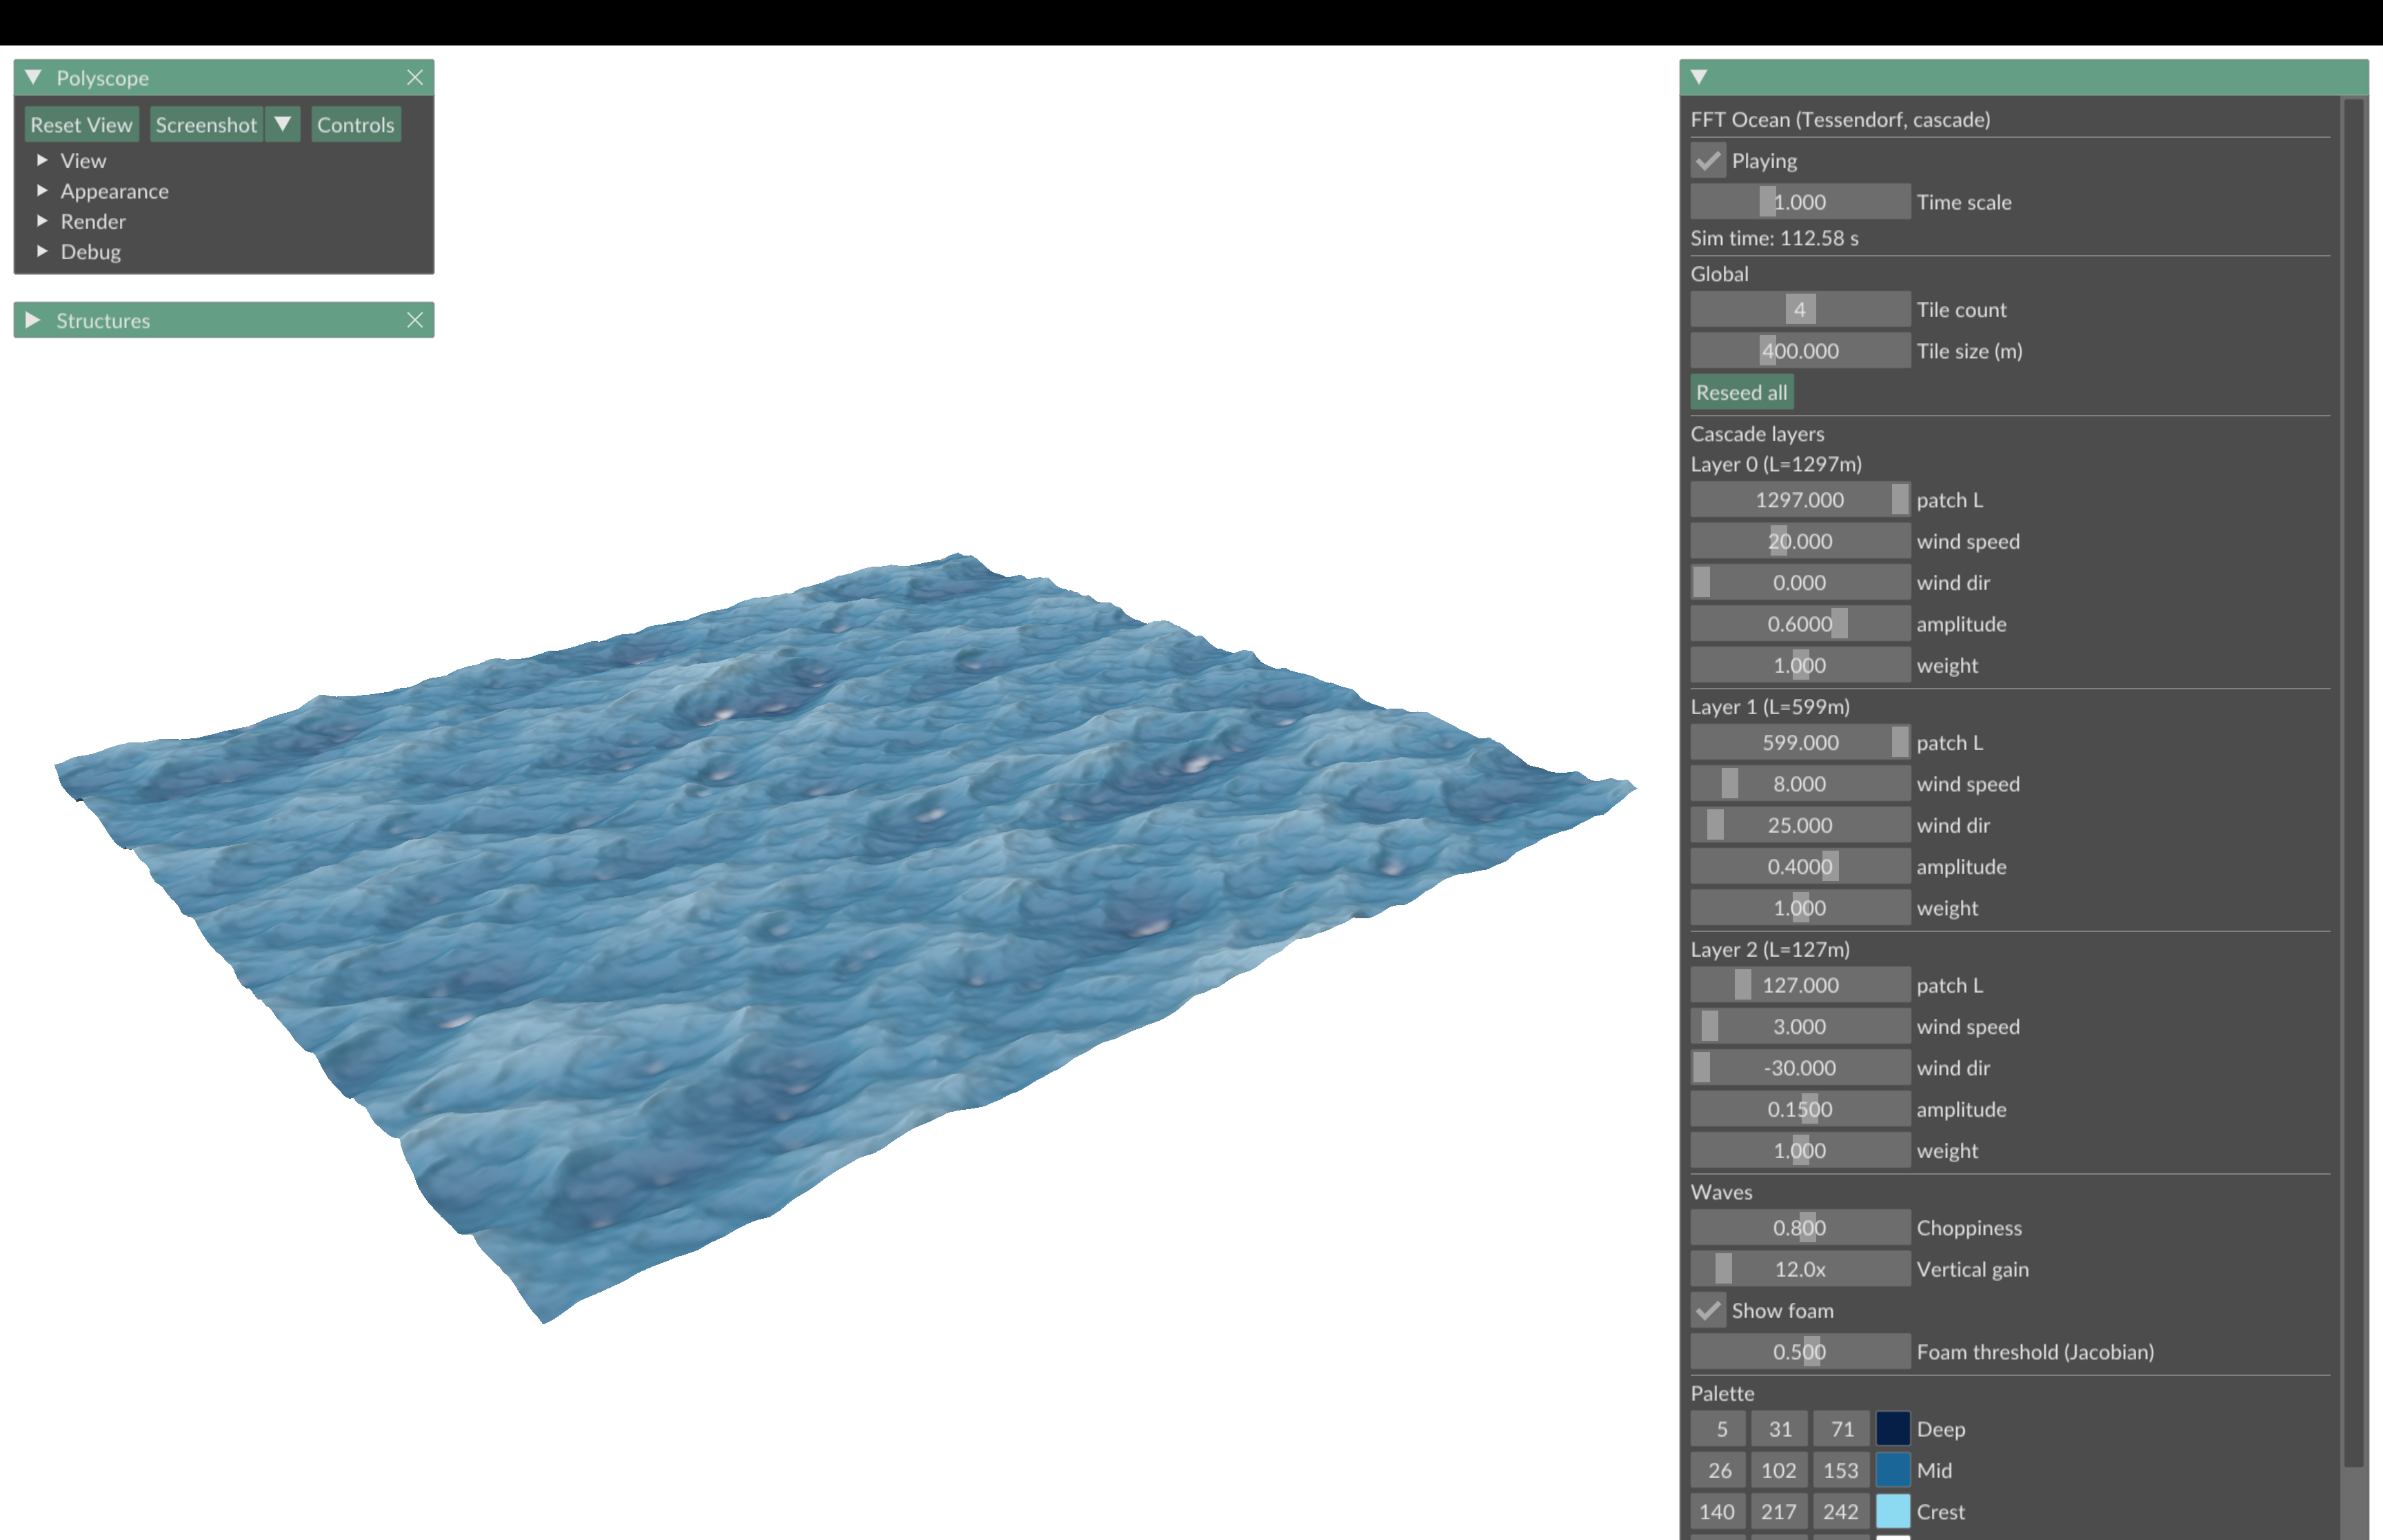
\includegraphics[width=\linewidth]{figs/ocean.png}
  \caption{Ocean preset, $V=20$\,m/s.}
\end{subfigure}\hfill
\begin{subfigure}[t]{0.48\textwidth}
  \centering
  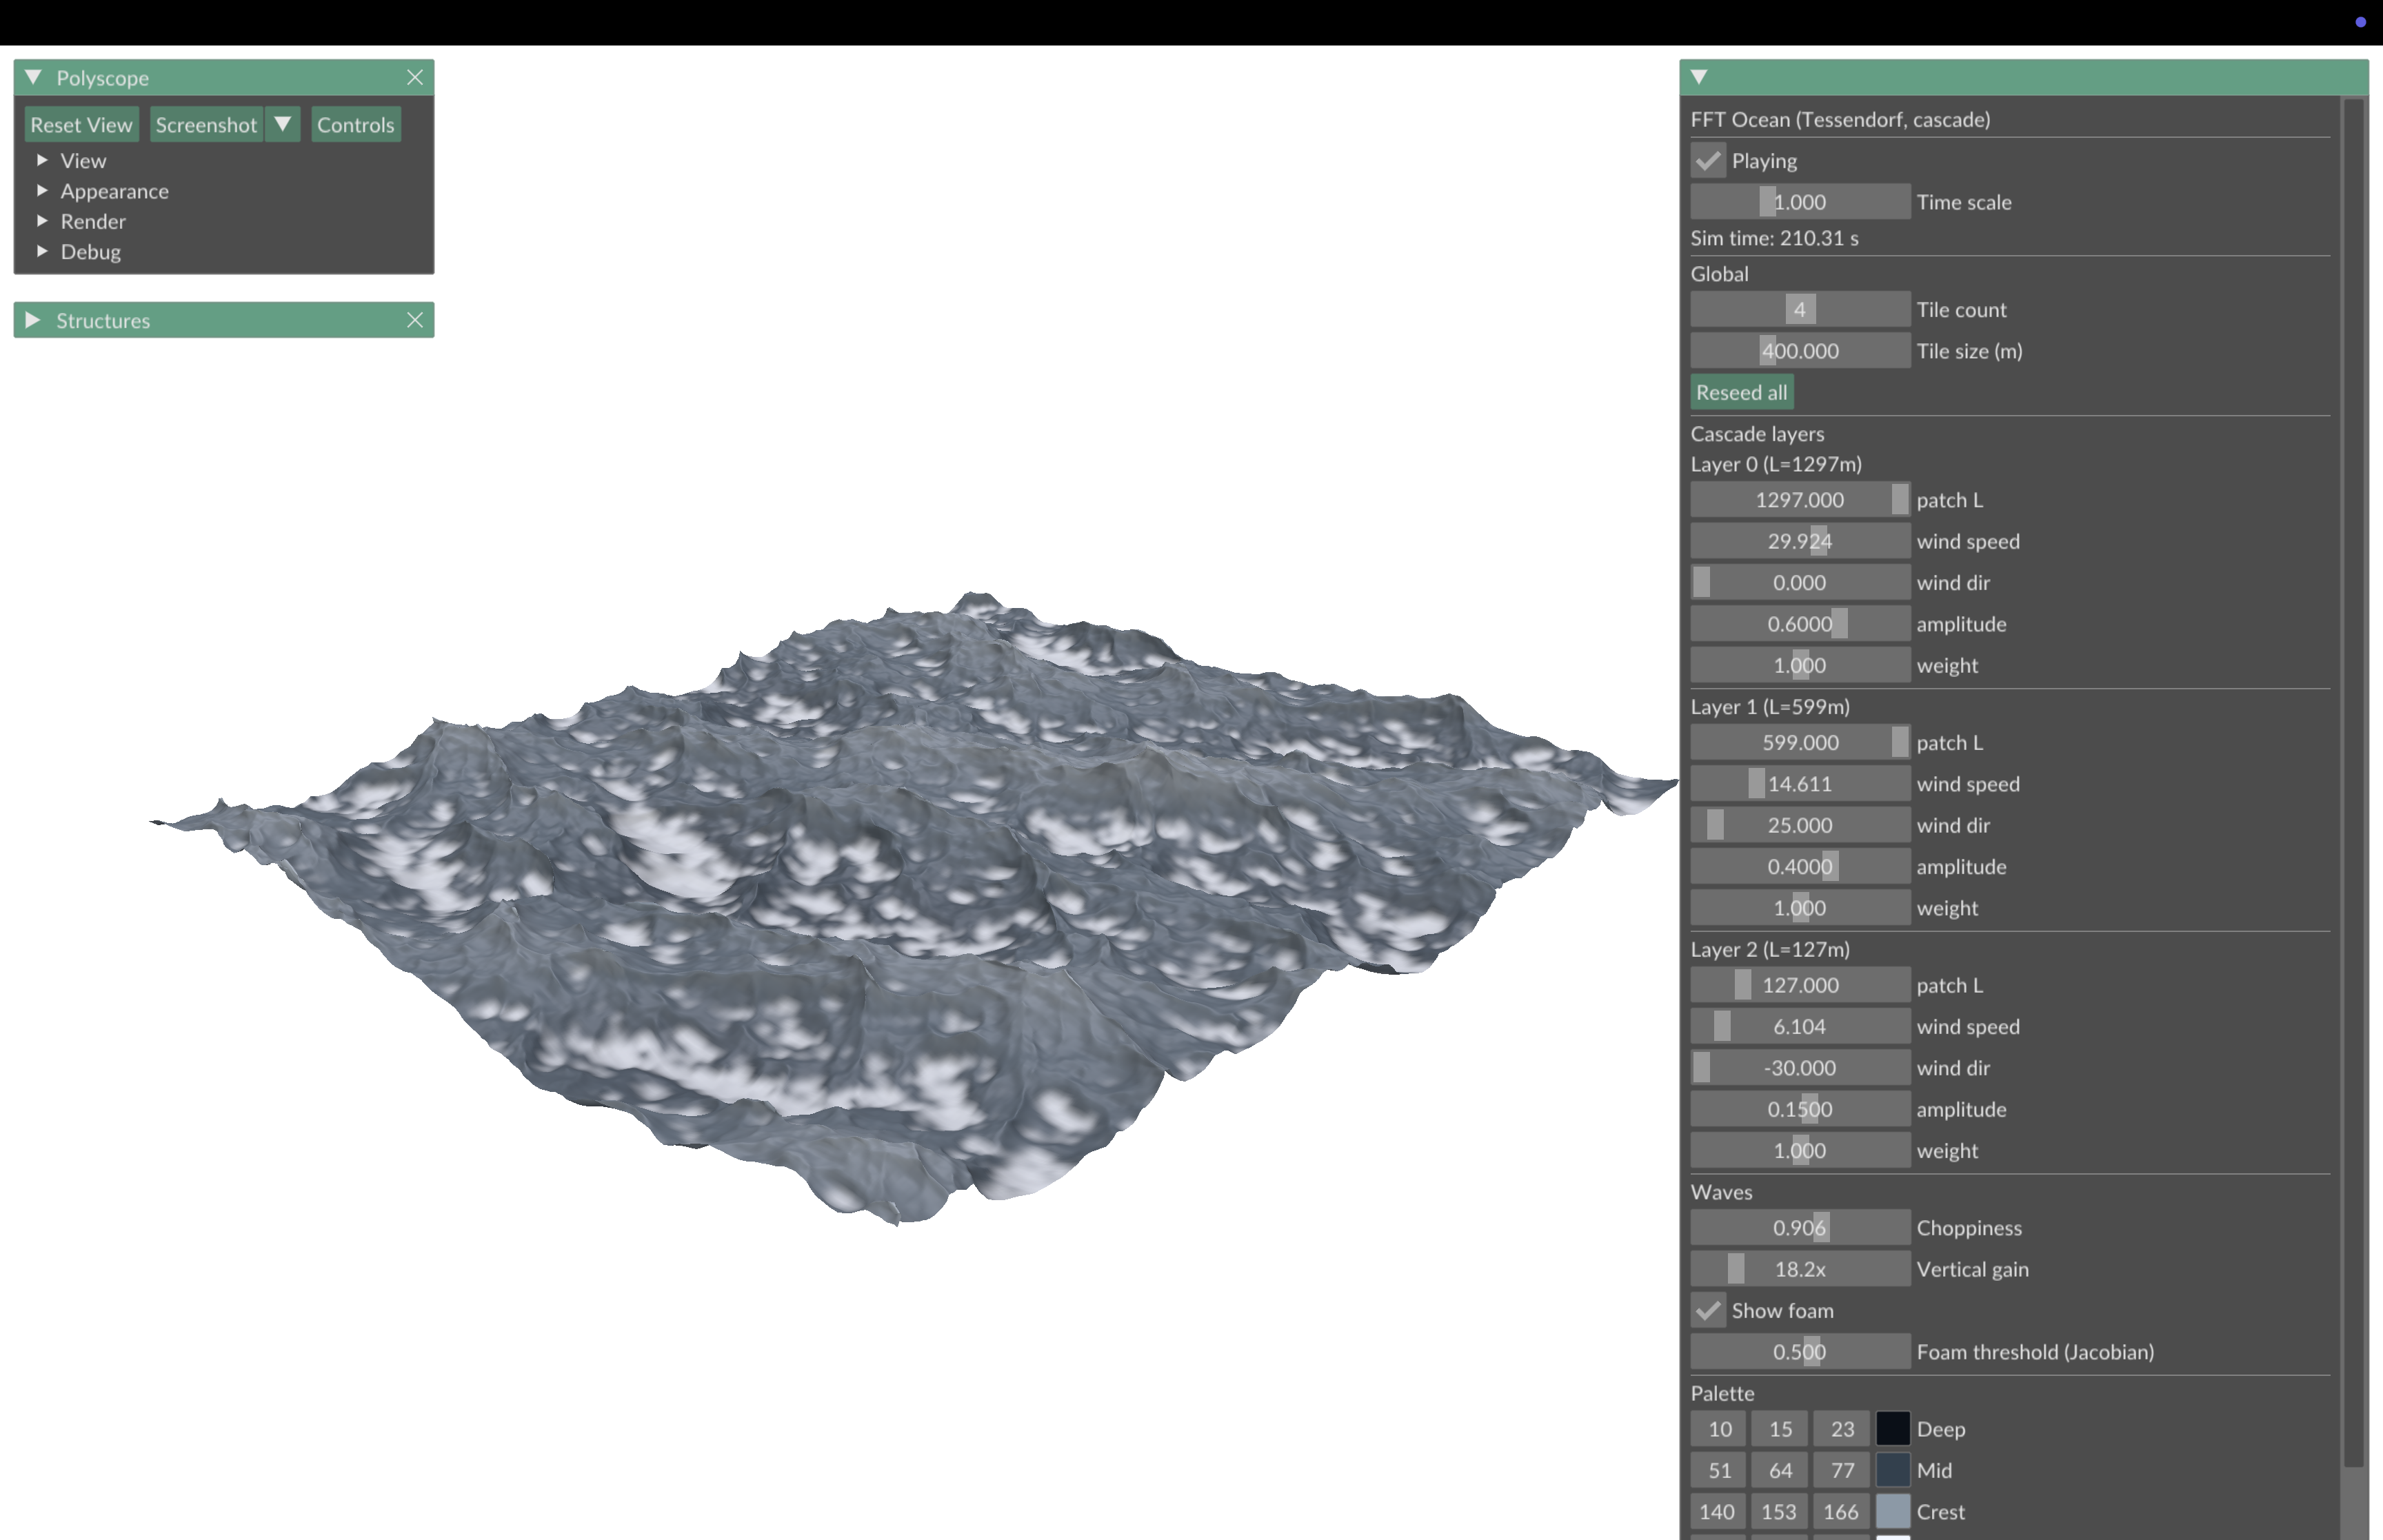
\includegraphics[width=\linewidth]{figs/storm.png}
  \caption{Storm preset, $V=35$\,m/s with high choppiness; foam concentrates on the forward face of breaking crests.}
\end{subfigure}\\[0.5em]
\begin{subfigure}[t]{0.48\textwidth}
  \centering
  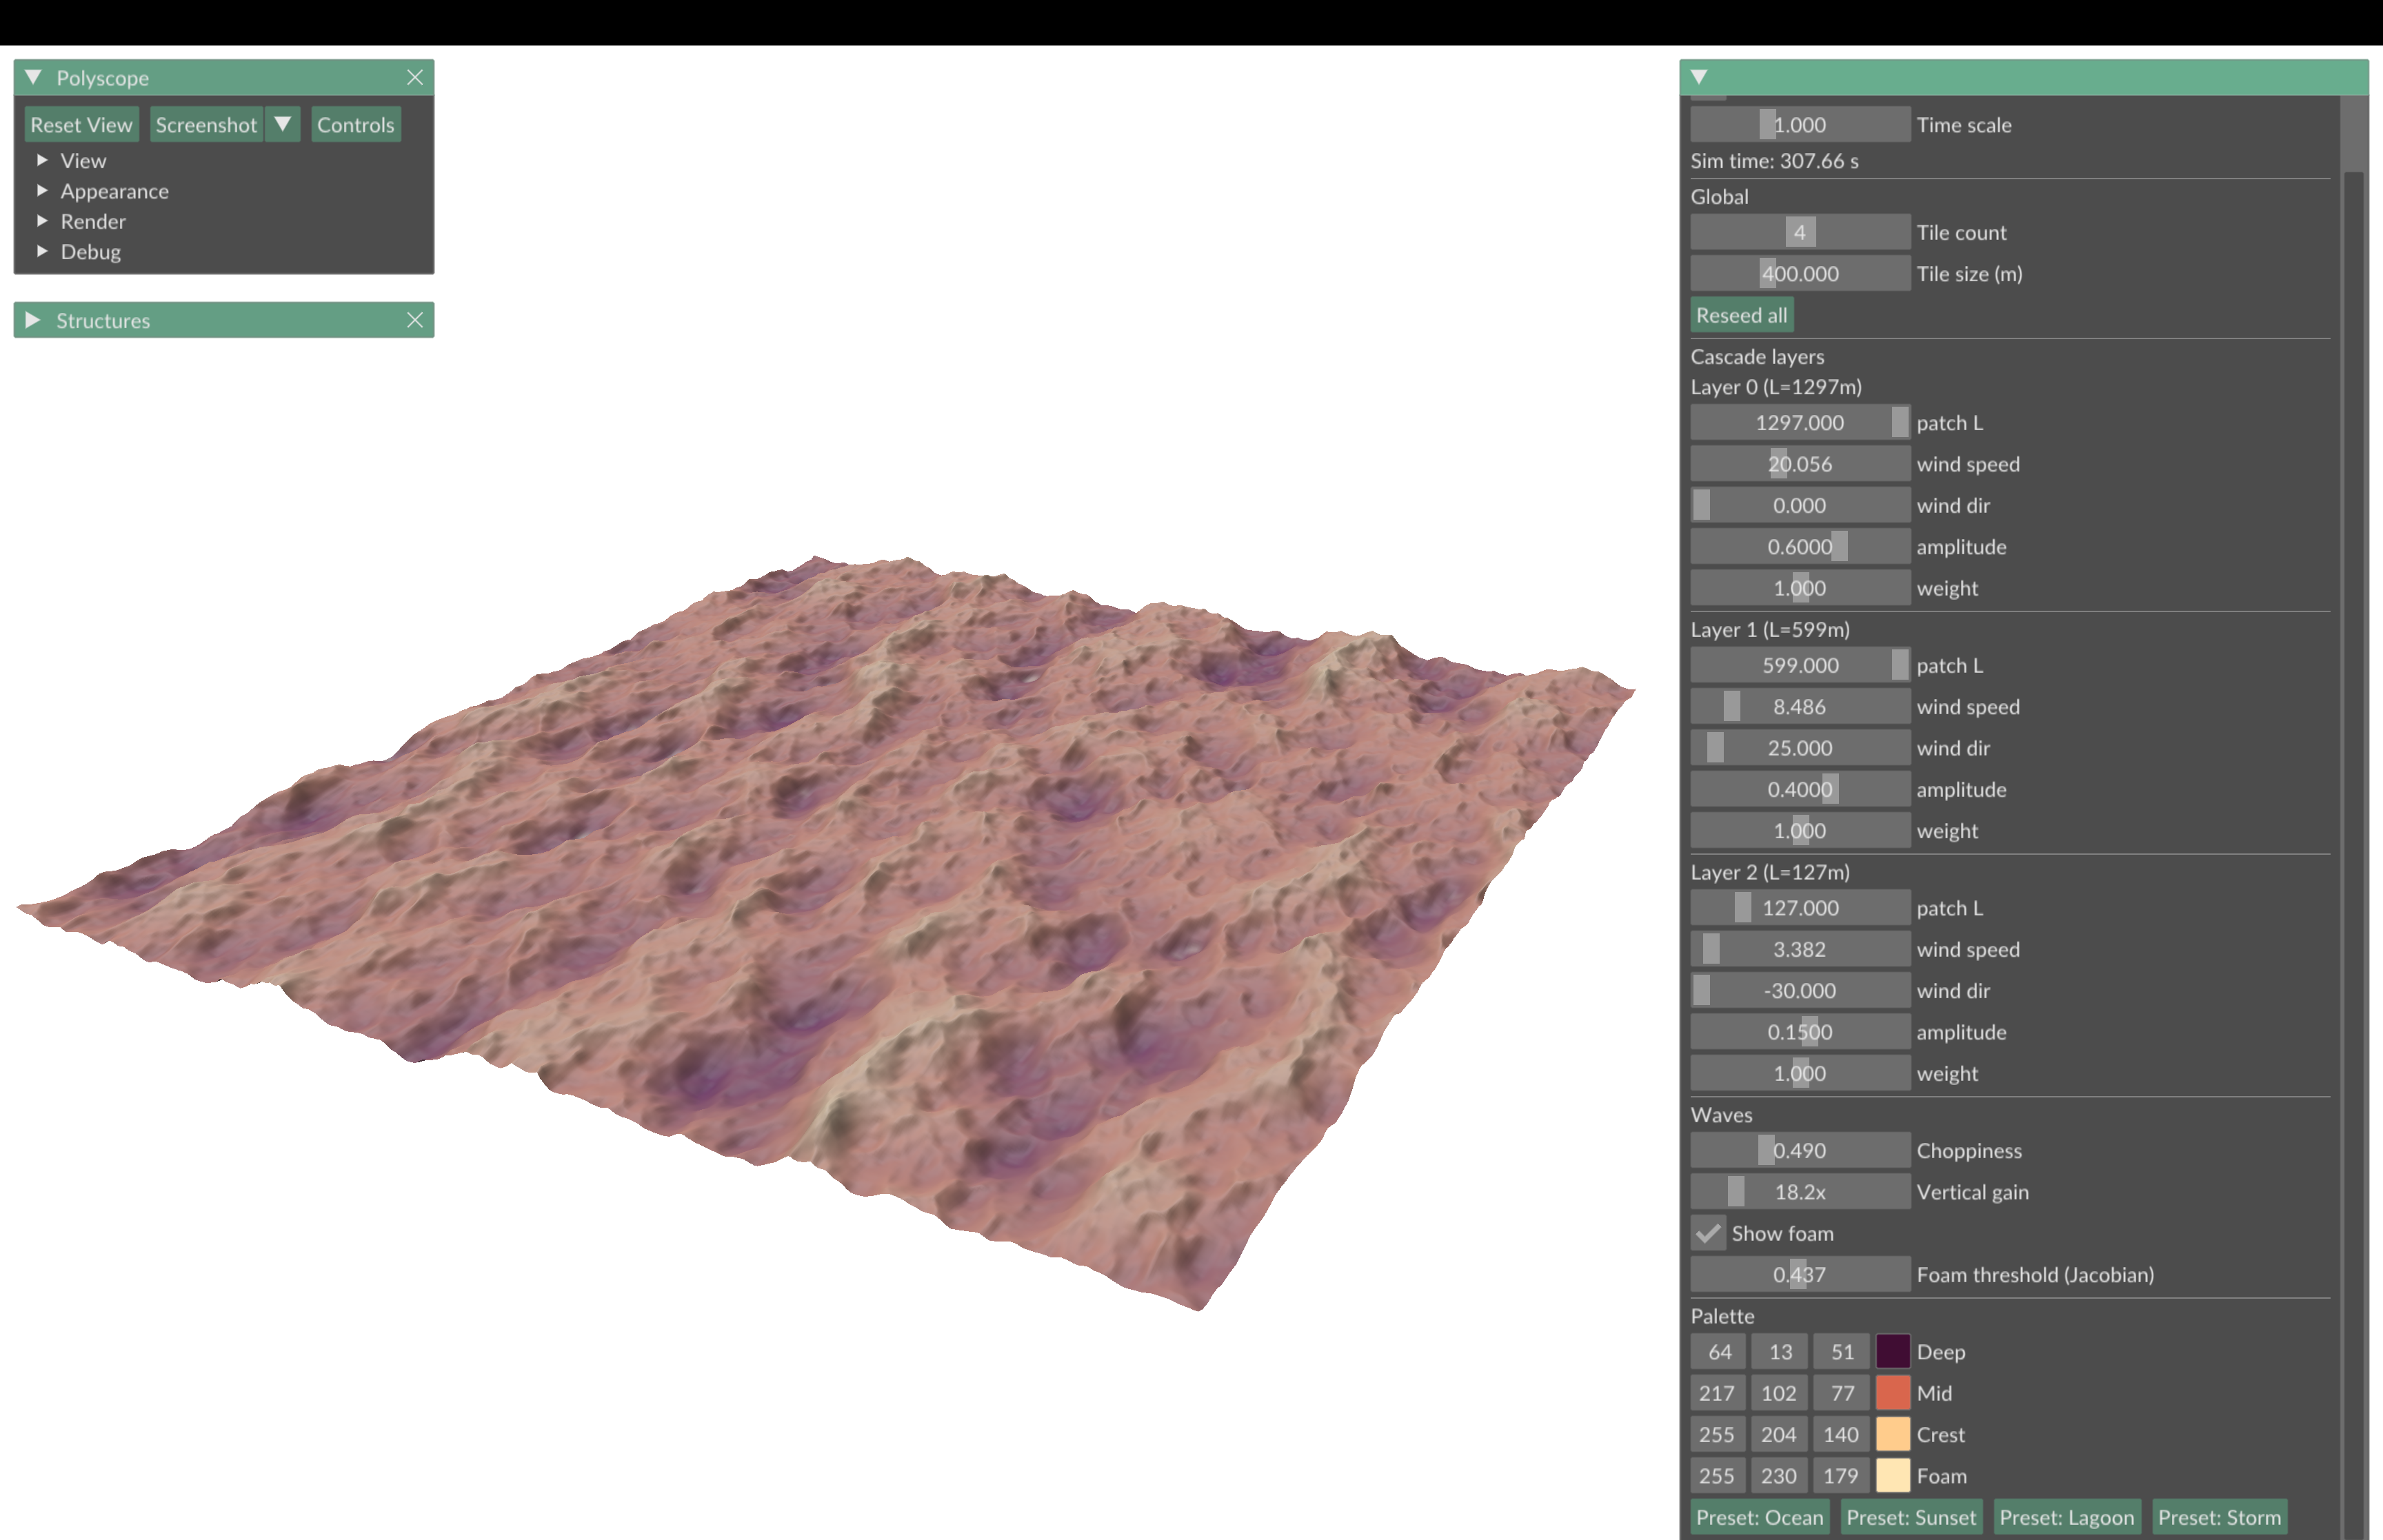
\includegraphics[width=\linewidth]{figs/sunset.png}
  \caption{Sunset palette over a moderate sea.}
\end{subfigure}\hfill
\begin{subfigure}[t]{0.48\textwidth}
  \centering
  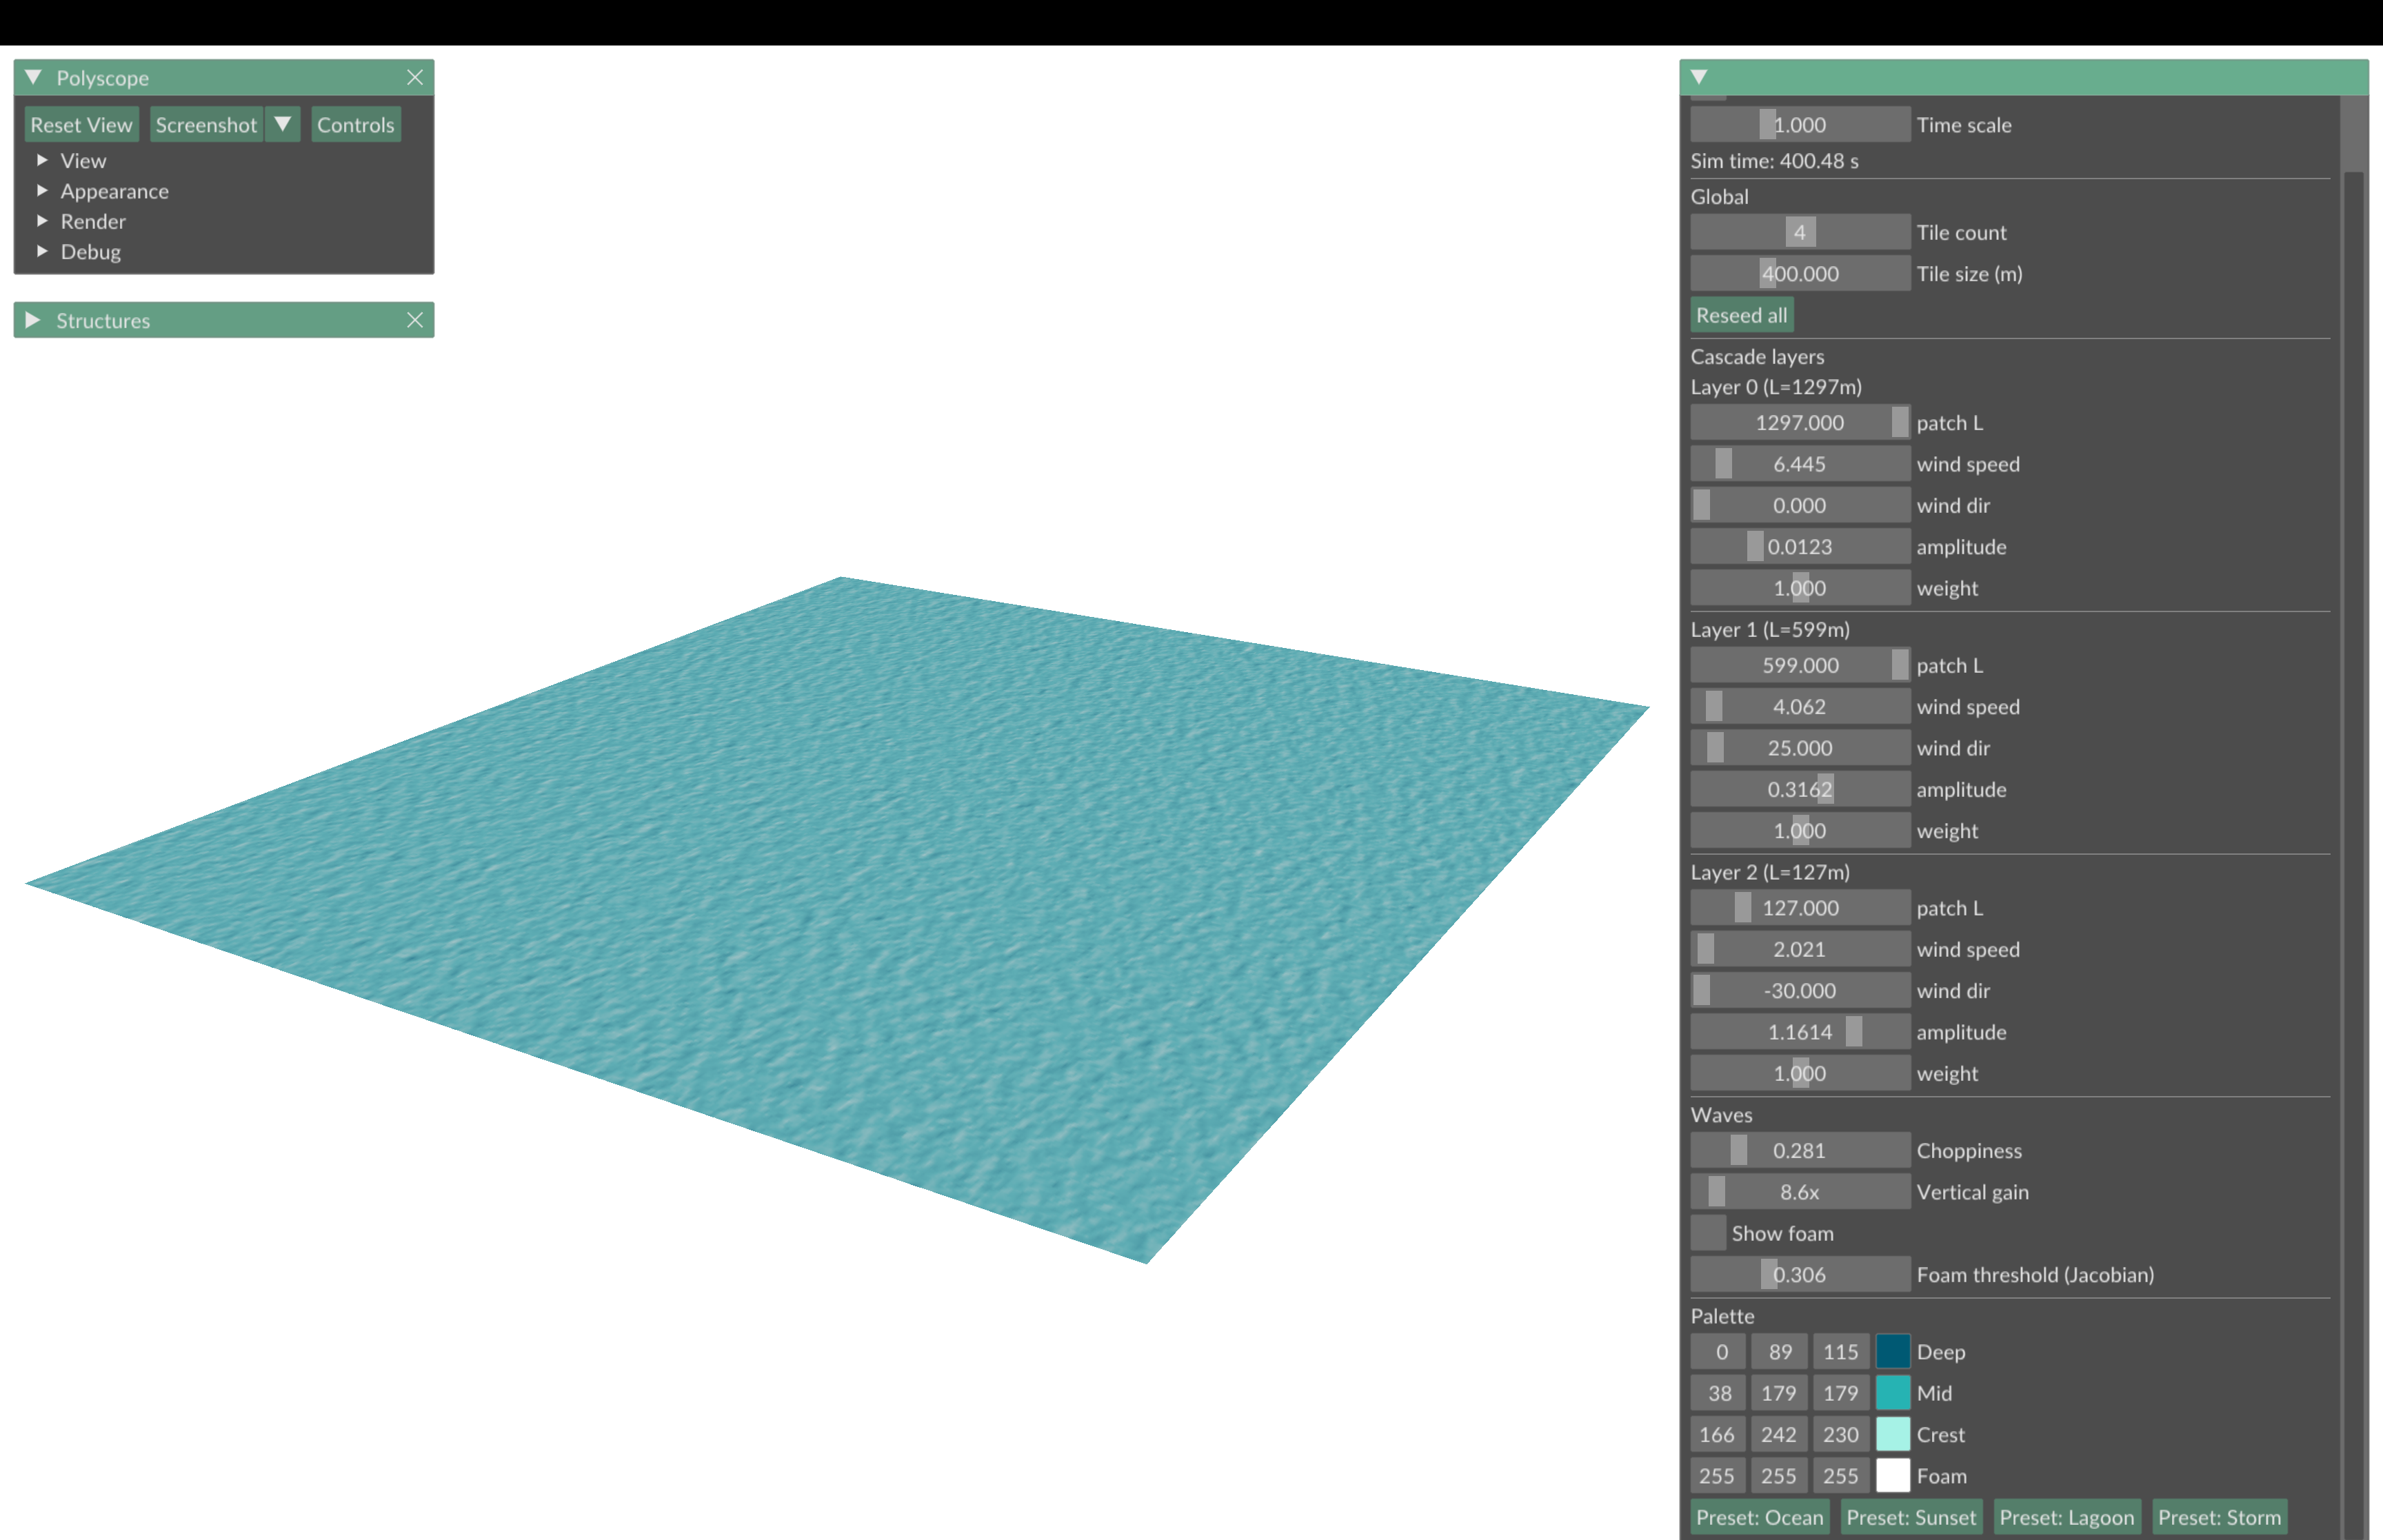
\includegraphics[width=\linewidth]{figs/lagoon.png}
  \caption{Lagoon palette, low wind: small ripples dominate.}
\end{subfigure}
\caption{Four presets driven by the same simulator with different wind, choppiness, and palette parameters.}
\end{figure}

\begin{thebibliography}{9}
\small
\bibitem{tessendorf} J. Tessendorf, ``Simulating Ocean Water,''
SIGGRAPH 2001 Course Notes, 2001.
\bibitem{horvath} C. J. Horvath, ``Empirical directional wave spectra for
computer graphics,'' \emph{Proc.\ DigiPro}, 2015.
\end{thebibliography}

\end{document}
